\documentclass{ximera}

\title{Vectoren in de fysica}
%\author{Daan Lipkens} %van KUL fysica vectoren

\begin{document}
\begin{abstract}
    Het verschil tussen scalaire en vectoriële grootheden, en de eigenschappen van vectoren.
\end{abstract}
\maketitle

\section{Scalaire versus vectoriële grootheden}

Heel wat grootheden in de fysica kunnen voorgesteld worden door een getalwaarde met een eenheid. Denk bijvoorbeeld aan het volume van een ton, de luchttemperatuur of het tijdstip van een gebeurtenis. Deze grootheden hebben een \textbf{scalair} karakter.

Maar vaak zijn enkel een getal en een eenheid niet voldoende om een grootheid precies te bepalen. Stel je wandelt in een dorp en je bent op zoek naar de supermarkt. Een voorbijganger laat je weten dat het in vogelvlucht nog $500\text{ m}$ wandelen is. Met deze info kan de supermarkt eender waar liggen op een cirkel met straal $500\text{ m}$. Om de exacte positie van de supermarkt te weten, moet ook de richting en de zin, bijvoorbeeld noordoosten, gegeven zijn. Pas als zowel de afstand als de richting gekend zijn, ligt de positie vast. Deze grootheid heeft een \textbf{vectorieel} karakter.

\begin{definition}[title={Scalaire en vectoriële grootheden}]\nl
    Fysische grootheden zijn ofwel `scalair' ofwel `vectorieel': 
    \begin{enumerate}
        \item \textbf{Scalaire grootheden} zijn volledig bepaald door een reëel getal en een eenheid. 
        Voorbeelden: massa $m$, lengte $\ell$, temperatuur $T$, \dots
        \item \textbf{Vectoriële grootheden} zijn volledig bepaald door een aangrijpingspunt, grootte (maatgetal met eenheid), richting en zin. 
        Voorbeelden: positie $\vec{r}$, snelheid $\vec{v}$, versnelling $\vec{a}$, kracht $\vec{F}$, elektrisch veld $\vec{E}$, \dots
    \end{enumerate}
\end{definition}

\section{Eigenschappen van vectoren}

Een vectoriële grootheid wordt genoteerd door een pijltje boven de letter: $\vec{a}$. De grootte van deze vector is een reëel getal (scalar) en noteren we als $a$ (dus het vectorsymbool zonder pijltje) of $\|\vec{a}\|$.

Een vector wordt grafisch voorgesteld door een pijl, waarvan de lengte evenredig is met zijn grootte. De rechte verbonden met de vector wordt de \textbf{drager} genoemd. De richting van deze drager komt overeen met de richting van de vectoriële grootheid (vb. horizontaal, verticaal, \dots). De zin van de vectorpijl is de zin waarin de vectoriële grootheid wijst (vb. links, rechts, \dots).

%---------------------------
% AFBEELDING: Drager van een vector
\begin{figure}[ht!]
    \captionsetup{width=0.85\textwidth}
    \begin{center}
        \begin{tikzpicture}[scale=1.5]
            % Drager
            \draw[dashed, gray, thick] (-1,0) -- (4,0) node[below, text=black] {\textit{drager}};
            % Vector
            \draw[->, thick, blue!70!black] (0,0) -- node[above, text=black] {$\vec{a}$} (1.5,0);
        \end{tikzpicture}
    \end{center}
    \caption{De drager van een vector $\vec{a}$.}
    \label{fig:drager_vector}
\end{figure}
%---------------------------

\begin{remark}[expandable=true,title={Vrije en gebonden vectoren}]\nl
    In de fysica maakt men een onderscheid tussen vrije en gebonden vectoren. Als je een vrije vector verschuift in het vlak of in de $3$-dimensionale ruimte, blijft dit dezelfde vector.
    
    Op een afbeelding stellen verschillende pijlen met dezelfde lengte, richting en zin \textit{dezelfde vrije vector} voor, maar \textit{verschillende gebonden vectoren}:
    \begin{enumerate}
        \item \textbf{Vrije vectoren} zijn gelijk als ze dezelfde lengte, richting en zin hebben. 
        \item \textbf{Gebonden vectoren} zijn gelijk als ze bovendien hetzelfde aangrijpingspunt hebben.
    \end{enumerate}
    Afhankelijk van het probleem (zoals bijvoorbeeld bij het berekenen van een krachtmoment) kunnen aangrijpingspunten essentieel zijn, en soms helemaal niet.
    
    %---------------------------
    % AFBEELDING: Vrije vectoren
    \captionsetup{width=0.85\textwidth}
    \begin{center}
        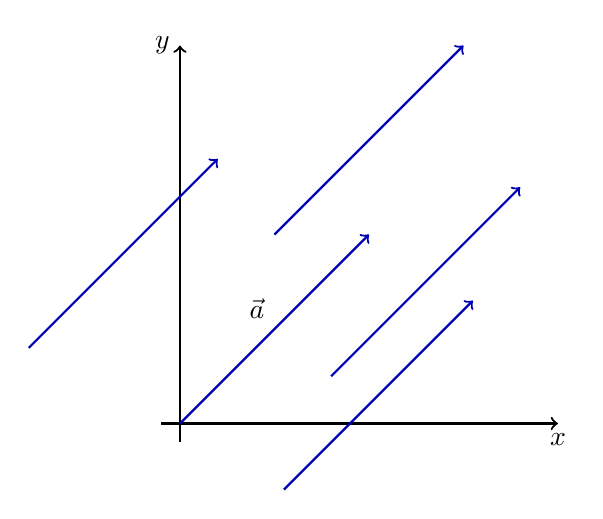
\begin{tikzpicture}[scale=1.2]
            % Assen
            \draw[->, thick] (-0.2,0) -- (4.0,0) node[below] {$x$};
            \draw[->, thick] (0,-0.2) -- (0,4.0) node[left] {$y$};
    
            % Vectoren stijl
            \tikzset{vec/.style={->, thick, blue!70!black}}
                
            % Vectoren
            \draw[vec] (0,0) -- node[above left, text=black] {$\vec{a}$} (2,2);
            \draw[vec] (1,2) -- (3,4);
            \draw[vec] (1.1,-0.7) -- (3.1,1.3);
            \draw[vec] (1.6,0.5) -- (3.6,2.5);
            \draw[vec] (-1.6,0.8) -- (0.4,2.8);
        \end{tikzpicture}
    \end{center}
    \captionof{figure}{Verschillende weergaven van dezelfde vrije vector $\vec{a}$.}
    \label{fig:vrije_vectoren}
    %---------------------------
\end{remark}

\end{document}